\subsubsection{固定背景与候选集合}
按假设（3），问题三读取经验证的问题二工作簿，固定其中 144 个活动计划和 15\,816 个已占用资源格，不在本问重新平移或撤销原计划。新增 C 类计划继承附件中的共同结构：频段宽度为 3，单次时长为 2，间隔时长为 8，使用次数为 12，因此相邻起点步长为 10。每个完整 C 类候选计划占用 \(3\times2\times12=72\) 个离散时频资源格。

在资源域 \([0,643)\times[0,100)\) 内，频段起点和首次时间起点分别满足
\[
f_0=0,1,\ldots,97,\qquad t_0=0,1,\ldots,531.
\]
因此完整候选起点总数为 \(98\times532=52\,136\)。逐个展开候选的 12 次使用事件并与固定问题二背景比较后，保留 2\,334 个无冲突候选。候选筛选没有抽样，也没有用剩余面积除以 72 代替完整模板检查。

图 \ref{fig:q3-candidate-layout} 用起点坐标展示这一筛选结果：浅色点是与冻结 Q2 背景不冲突的 2\,334 个候选，深色点是最终选中的 141 个新增计划。图中位置只表示候选起点，不把起点密度误读为优化目标。

\begin{figure}[htbp]
  \centering
  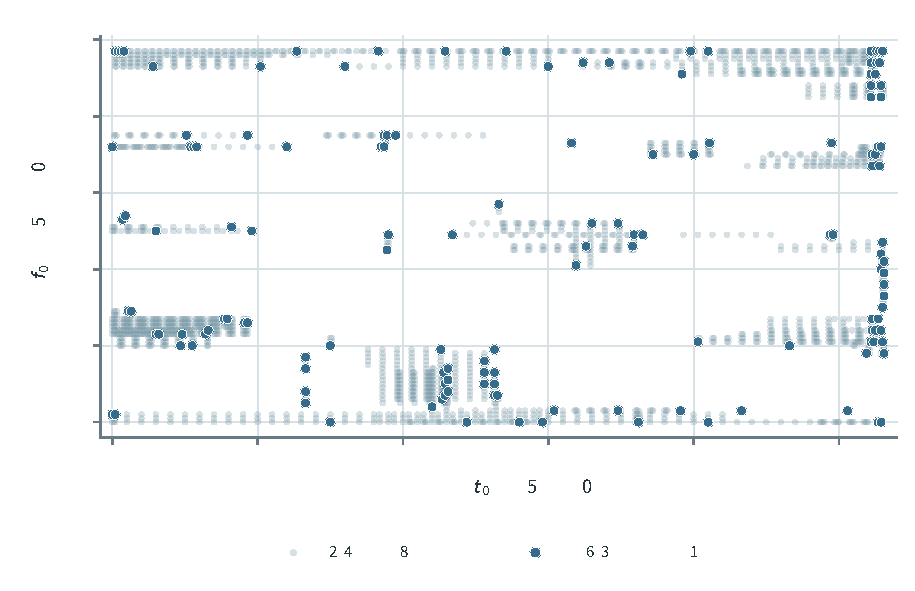
\includegraphics[width=0.92\textwidth]{figures/fig5_q3_candidate_layout.pdf}
  \caption{固定问题二条件下的 C 类候选起点与选中方案}
  \label{fig:q3-candidate-layout}
\end{figure}

\subsubsection{集合装填模型}
对每个合法候选 \(p\) 定义二元变量 \(y_p\)，令 \(\mathcal K_p\) 为其完整资源格集合，最大化新增计划数量：
\begin{equation}
\max\sum_{p}y_p,
\qquad
\sum_{p:\,c\in\mathcal K_p}y_p\le 1-O_c,
\quad c\in\mathcal C,
\label{eq:q3-set-packing}
\end{equation}
其中 \(O_c\) 表示固定问题二方案对资源格 \(c\) 的占用。主模型包含 2\,334 个候选变量、15\,521 条被候选使用的资源格约束和 168\,048 个非零系数。

\subsubsection{最大新增数量}
集合装填模型返回 141 个新增计划，HiGHS 求解器\cite{highs} 状态为 \texttt{OPTIMAL}，下界和上界均为 141，MIP gap 为 0。为避免结论依赖单一约束编码，又将 2\,334 个候选改写为候选两两冲突模型；若两个候选共享任一资源格，则加入
\[
y_p+y_q\le 1.
\]
该独立模型含 66\,472 条成对冲突约束，同样得到 141。进一步加入 \(\sum_p y_p\ge142\) 后模型不可行，因此“141 台可行”和“142 台不可行”共同闭合了固定背景下的最大新增数量。

\begin{table}[H]
\centering
\caption{问题三候选筛选与最大性验证}
\label{tab:q3-result}
\begin{tabular}{lr}
\toprule
项目 & 数值 \\
\midrule
完整 C 类候选起点 & 52\,136 \\
与固定 Q2 背景不冲突的候选 & 2\,334 \\
集合装填模型下界/上界 & 141/141 \\
独立成对冲突模型下界/上界 & 141/141 \\
新增计划数 & 141 台 \\
\bottomrule
\end{tabular}
\end{table}

\subsubsection{合并结果与边界}
141 台新增计划占用 10\,152 个资源格，与固定问题二方案合并后形成 285 个活动计划，占用 25\,968 个不同资源格。连续半开区间检查和离散资源格检查均未发现 Q2--Q3 间冲突或新增计划之间的冲突，\texttt{result3.xlsx} 的 141 行与结果 JSON 逐行一致。

“最多新增 141 台”依赖三个条件：当前批准的具体问题二方案、资源域 \([0,643)\times[0,100)\) 以及附件 C 类共同模板。改变任一条件都需要重新生成候选集合并求解，不能将 141 台推广到任意问题二方案。

\subsubsection{问题三小结}
在固定问题二方案下，完整候选枚举与两种独立冲突编码均支持最多新增 141 台 C 类装备；该结果是条件最优结论，且其适用边界已经明确。
